%\VignetteIndexEntry{Analysis of Flow Cytometry Bead Data}
%\VignetteDepends{flowBeads}
%\VignetteKeywords{}
%\VignettePackage{flowBeads}
\documentclass[11pt]{article}




\newcommand{\scscst}{\scriptscriptstyle}
\newcommand{\scst}{\scriptstyle}
\newcommand{\Rfunction}[1]{{\texttt{#1}}}
\newcommand{\Rcode}[1]{{\texttt{#1}}}
\newcommand{\Robject}[1]{{\texttt{#1}}}
\newcommand{\Rpackage}[1]{{\textsf{#1}}}
\newcommand{\Rdata}[1]{{\textsf{#1}}}
\newcommand{\Rclass}[1]{{\textit{#1}}}



\title{flowBeads: Bead Normalisation in Flow Cytometry} 
\date{\today}



\usepackage[text={7.5in,9in},centering]{geometry}
\usepackage{Sweave}
\setkeys{Gin}{width=0.95\textwidth}
\usepackage[round]{natbib}

\usepackage{graphicx}
\usepackage{url}
\usepackage{hyperref} 
\usepackage{amsmath}


% \usepackage{setspace}
% \setlength{\parindent}{0in}



\begin{document}
\Sconcordance{concordance:HowTo-flowBeads.tex:HowTo-flowBeads.Rnw:%
1 55 1 1 4 54 1 1 2 4 0 1 2 1 12 22 0 1 2 2 1 1 2 4 0 1 2 27 1 1 2 1 0 %
1 1 3 0 1 2 4 1 1 2 1 0 1 1 3 0 1 2 4 1 1 2 26 0 2 2 6 0 1 1 5 0 1 1 6 %
0 1 1 6 0 1 2 19 1 1 2 1 0 1 1 3 0 1 2 5 1 1 2 1 0 1 1 3 0 1 2 4 1 1 2 %
4 0 1 2 1 4 2 1 1 2 4 0 1 2 8 1 1 2 11 0 1 2 1 5 5 1 1 2 1 0 1 1 5 0 1 %
1 6 0 1 2 1 20 4 1 1 2 4 0 1 2 17 1 1 2 1 0 1 1 7 0 2 2 1 0 3 1 3 0 1 2 %
1 20 6 1 1 2 4 0 1 2 56 1}

\maketitle

\begin{abstract}
    The \Rpackage{flowBeads} package is an extension of \Rpackage{flowCore} for bead data.
    It provides basic functionality for loading, gating and doing normalisation with bead data.
    Beads specially manufactured to known fluoresence,  defined in terms of standard units of fluorescence, are routinely run in flow cytometry
    for the purpose of instrument quality control and normalisation.
    The transformation of measured intensity (Mean Fluorescence Intensity) to standard units of fluorescence,
    Molecules of Equivalent Fluorochrome, allows for sensible comparison of data acquired on different days and on different instruments.
    The parameters of the transform also correspond to basic quality control estimates of the detector linearity and the background.
\end{abstract}




\section{Theory}

The expected fluorescent signal of a bead is determined by:
\begin{itemize}
    \item the amount of fluorochrome carried by the bead
    \item the properties of the excitation source (wavelength of laser)
    \item the properties of the detector channel (bandpass and voltage)
\end{itemize}
Given these properties, the \textbf{Molecules of Equivalent Fluorochrome (MEF)} or Molecules of Equivalent Soluble Fluorochrome (MESF)
standard unit of fluorescence is calculated by the manufacturer.
This theoretical value provides an absolute scale for measuring fluorescence 
to compare samples analysed at different times or under different laser/detector configurations \citep{Schwartz:1996,Dendrou:2009}.
The transform from relative fluorescence to standard fluorescence is a linear transform which is estimated 
by linear regression of the \textbf{Mean Fluorescence Intensity (MFI)} of beads belonging to a number (usually six) of different populations
of increasing brightness against their expected MEF fluorescence.
Since the MEF of the bead populations scales multiplicatively, a chosen transform \texttt{f} is appropriate to linearise the data.
In the case of FCS2 data, \texttt{f} is $\text{log}_{10}$, and in the case of FCS3, the default choice is the \Rfunction{logicleTransform} of the \Rpackage{flowCore}
package.
On the \texttt{f} linearised fluorescence scale the transform is therefore:

\[
\text{f}(\text{MEF}) = \beta \times \text{f}(\text{MFI}) + \alpha
\]

\[
\text{MEF} = \text{f}^{-1} ( \beta \times \text{f}(\text{MFI}) + \alpha )
\]

In the special case where the transform \texttt{f} is $\text{log}_{10}$, this can be further simplified to:

\[
\text{MEF} = 10^\alpha \times \text{MFI}^\beta 
\]


Provided the linearity of the detector is good, the $\beta$ parameter, representing the slope, is generally close to one.
When the beads are run on different days, the MFIs of the bead populations move little relative to each other but instead shift together as a whole,
thus the intercept $\alpha$, which can be interpreted as the background fluorescence, varies more than the the slope $\beta$.
%In fact, \citet{Dendrou:2009}  assumed in their MEF transform that $\beta=1$ and only estimated the $\alpha$ parameter.

In order to apply the MEF transform, the MEF of the beads for a given laser/detector setup, as supplied by the manufacturer, 
needs to be matched to the laser/detector configuration provided in the FCS bead file.
However, since not all required laser/detector properties are stored as part of the FCS 2 or 3 file format,
we rely instead on the names of the detectors channels in the FCS file matching those in the MEF configuration file.
As part of the \Rpackage{flowBeads} package,
there is support for 
\textbf{Dakocytomation FluoroSpheres} beads (see Table 1)
and
\textbf{ThermoFischer Scientific Cytocal} 
for the standard \textbf{LSRII} and \textbf{LSRFortessa} laser/detector setup,
but any other type of bead can be supported provided the MEF configuration file is specified.
\noindent
And to load the Dakocytomation configuration file into the current workspace:
\begin{Schunk}
\begin{Sinput}
> data(dakomef)
\end{Sinput}
\end{Schunk}

% latex table generated in R 2.14.2 by xtable 1.7-0 package
% Wed Mar 13 01:06:55 2013
\begin{table}[ht]
\begin{center}
\begin{tabular}{rrrrrr}
  \hline
 & FITC & PE & PE.CY5 & APC & PE.TEXAS.RED \\ 
  \hline
1 &  &  &  &  &  \\ 
  2 & 2500 & 1500 & 750 & 4100 & 552 \\ 
  3 & 6500 & 4400 & 2100 & 10300 & 2014 \\ 
  4 & 19000 & 14500 & 6900 & 25500 & 6975 \\ 
  5 & 55000 & 43800 & 22100 & 67300 & 20685 \\ 
  6 & 150000 & 131200 & 77100 & 139100 & 71888 \\ 
   \hline
\end{tabular}
\caption{
             FluoroSpheres from Dakocytomation.
             The Molecules of Equivalent Fluorochromes (MEF) values for the six bead populations as provided by the manufacturer
             for the LSRII.
             The first bead population are blank as they contain contain no flurochrome by design.
             }
\end{center}
\end{table}
\noindent
To load the Cytocal configuration file into the current workspace:
\begin{Schunk}
\begin{Sinput}
> data(cytocalmef)
\end{Sinput}
\end{Schunk}

Note that the underlying assumption in using beads as a reference is that the physical MEF property of these beads is more stable
than the detected MFI of the bead population as reported by the instrument.
For this to be true, the quality of the beads must not be compromised by age or poor storage. 
Also it is important to keep in that in mind that if any properties of the laser/detector change, for example the voltage of the detector,
then the beads need to be run again to recompute the correct transform.


%Calibration can be accomplished by tweaking the parameters of the instrument so that the recorded MFI is always the same across days.
%However this method is quite coarse and may lead to other undesired effects.
%The preferred approach is instead to keep the instrumental parameters stable and instead use the beads to measure the change in the MFIs of the bead populations and apply a transformation to normalise the data.

%The instrument we used is the LSR II from BD Bioscience.
%<<<instrument>>=
%data(gbeads1)
%gbeads1@description[['$CYT']]
%@


%LSRII setup
%Lasers: Blue 488; Red 633; Violet 405
%Detectors: "FITC";"PE 575/26";"PE-Tx Red 610/20";"PerCP/Cy5.5 695/40";"PE Cy5 695/40";"PE Cy5 660/20";"PE Cy7 780/60";"APC 660/20";"AlexaFluor 700 730/45";"APC Cy7 780/60";"Pac Blue 440/50";"Pac Orange 525/50"

\section{Loading Bead Files}

Two example FCS 3 bead files, Dakocytomation beads ran on two different days, are included as part of the \Rpackage{flowBeads} package.
These files may be loaded like so:

\begin{Schunk}
\begin{Sinput}
> beads1 <- BeadFlowFrame(fcs.filename=system.file('extdata', 'beads1.fcs', package='flowBeads'))
> beads2 <- BeadFlowFrame(fcs.filename=system.file('extdata', 'beads2.fcs', package='flowBeads'))
\end{Sinput}
\end{Schunk}

\noindent
As no MEF configuration file has been specified as an argument to \Rcode{BeadFlowFrame}, they are assumed to be the default Dakocytomation beads.
\Rcode{beads1} and \Rcode{beads2} are also saved as R objects as part of the \Rpackage{flowBeads} package and so can be loaded directly:

\begin{Schunk}
\begin{Sinput}
> data(beads1)
> data(beads2)
\end{Sinput}
\end{Schunk}

\noindent
%\Rclass{BeadFlowFrame} is an extension of \Rclass{flowFrame}.
Here are a few ways of extracting information from \Rclass{BeadFlowFrame} objects:

\begin{Schunk}
\begin{Sinput}
> print(beads1)
\end{Sinput}
\begin{Soutput}
BeadFlowFrame object '9de89faa-c6fe-4d82-ad9b-ae64a02c3122'
from 2008-01-21
with 5144 beads and 8 observables:
            name desc  range minRange maxRange
$P1          FSC <NA> 262144     0.00   262143
$P2          SSC <NA> 262144     0.00   262143
$P3    ALEXA.488 <NA> 262144   -82.08   262143
$P4       PE.CY7 <NA> 262144   -87.78   262143
$P5          APC <NA> 262144   -26.60   262143
$P6           PE <NA> 262144  -111.00   262143
$P7    ALEXA.700 <NA> 262144   -77.90   262143
$P8 PACIFIC.BLUE <NA> 262144     0.00   262143
146 keywords are stored in the 'description' slot
Beads MEF
    FITC    RPE RPE.CY5    APC PE.TEXAS.RED
1   2500   1500     750   4100          552
2   6500   4400    2100  10300         2014
3  19000  14500    6900  25500         6975
4  55000  43800   22100  67300        20685
5 150000 131200   77100 139100        71888
\end{Soutput}
\end{Schunk}

\begin{Schunk}
\begin{Sinput}
> print(length(beads1))
\end{Sinput}
\begin{Soutput}
[1] 5144
\end{Soutput}
\begin{Sinput}
> print(getDate(beads1))
\end{Sinput}
\begin{Soutput}
[1] "2008-01-21"
\end{Soutput}
\begin{Sinput}
> print(getParams(beads1))
\end{Sinput}
\begin{Soutput}
[1] "ALEXA.488"    "PE.CY7"       "APC"          "PE"           "ALEXA.700"   
[6] "PACIFIC.BLUE"
\end{Soutput}
\begin{Sinput}
> print(getMEFparams(beads1))
\end{Sinput}
\begin{Soutput}
[1] "FITC"         "RPE"          "RPE.CY5"      "APC"          "PE.TEXAS.RED"
\end{Soutput}
\end{Schunk}


\noindent
Once the bead files are loaded we can then gate them to identify the distinct populations and compute the MEF transform.


\section{Gating Bead Data}

%Beads are manufactured to the same size so provided clumping of beads is rare it is straightforward to identifiy the main population of singlet beads by gating on forward and side scatter.
Gating of bead data is straightforward as the number of bead populations is known a priori.
In the forward and side scatter detector channels, a single population is expected since all beads are known to be of identical shape and size.
Using the \Rfunction{norm2Filter} from \Rpackage{flowCore} \citep{rpackage:flowcore},
we fit a bivariate Gaussian to the data.
Events lying more than one standard deviation away from the mean of the main bead population are excluded.% as not being singlets.

Once we have gated on the main bead population in the scatter channels, we know from the MEF file that the beads belong to six populations of increasing brightness.
All channels are gated with the number of expected clusters set to the number of bead population reported in the bead type file
(which is six in the case of Dakocytomation beads).
The gating is done separately on each fluorescent channel using the \Rfunction{pam} function in the \Rpackage{cluster} \citep{rpackage:cluster} which is an implementation of the K-medoids algorithm:

\begin{Schunk}
\begin{Sinput}
> gbeads1 <- gateBeads(beads1, verbose=T)
> gbeads2 <- gateBeads(beads2, verbose=F)
\end{Sinput}
\end{Schunk}

\noindent
Note \Rfunction{gateBeads} is quite a slow function as the \Rfunction{pam} function is quite computationally intensive.
\Rcode{gbeads1} and \Rcode{gbeads2} are \Rclass{GatedBeadFlowFrame} objects which contain the results of the gating.
They can also be loaded directly as saved R objects:

\begin{Schunk}
\begin{Sinput}
> data(gbeads1)
> data(gbeads2)
\end{Sinput}
\end{Schunk}

\noindent
%The K-medoids algorithm computes a complete distance matrix which makes it quite
To visualise the results of the gating (see Figure \ref{gbeads1plot} for \Robject{gbeads1} and Figure \ref{gbeads2plot} for \Robject{gbeads2}):

\begin{Schunk}
\begin{Sinput}
> plot(gbeads1)
\end{Sinput}
\end{Schunk}


\noindent
Individual channels can be plotted like so:
\begin{Schunk}
\begin{Sinput}
> plot(gbeads1, 'APC')
\end{Sinput}
\end{Schunk}

\noindent
Clustering statistics are also calculated and stored in the \Robject{clustering.stats} slot as
a three way array indexed
by statistic (count, mean, standard deviation, coefficient of variation),
channel (\texttt{ALEXA.488, PEC.Y7, APC, PE, ALEXA.700} and \texttt{PACIFIC.BLUE})
and bead population (one to six).
For example, the clustering stats of bead population one (the blank beads):

\begin{Schunk}
\begin{Sinput}
> gbeads1@clustering.stats[,,1]
\end{Sinput}
\begin{Soutput}
        ALEXA.488     PE.CY7       APC        PE ALEXA.700 PACIFIC.BLUE
count   156.00000  359.00000 156.00000 156.00000 156.00000    156.00000
mean.fi  14.30846  -11.04752 116.98397  11.06385  34.69327    171.85102
sd.fi    33.59705   23.40036  58.69615  44.54962  60.68674     35.99458
cv      234.80550 -211.81550  50.17452 402.65946 174.92368     20.94522
\end{Soutput}
\end{Schunk}


The \Rclass{GatedBeadFlowFrame} defines \Robject{mef.transform} slot which contains a list indexed by channel
name, where each element is a list containing the transformation function to apply as well as the coefficients of the transform.
As we do not have MEF values for all detector channels, we only define an MEF transform for ones with matching names in the bead configuration file (in this case APC).
See Figure \ref{fig:absoluteNormalisation} for absolute normalisation of the APC channel.

\begin{Schunk}
\begin{Sinput}
> mef.transform <- gbeads1@mef.transform
> names(mef.transform)
\end{Sinput}
\begin{Soutput}
[1] "APC"
\end{Soutput}
\begin{Sinput}
> names(mef.transform$APC)
\end{Sinput}
\begin{Soutput}
[1] "alpha" "beta"  "m"     "rse"   "fun"  
\end{Soutput}
\end{Schunk}


\noindent
The \Rcode{toMEF} function takes a \Rclass{GatedBeadFlowFrame} and a \Rclass{flowFrame} and normalises the channels
for which we have an MEF transform:

\begin{Schunk}
\begin{Sinput}
> toMEF(bead.data, flow.data)
\end{Sinput}
\end{Schunk}

\section{Relative Normalisation}

The MEF provides an absolute reference but we can still normalise in the absence of MEF provided we can align the MFIs across days.
An advantage of relative normalisation is that we can also align the blank bead population as we do not need the MEF.
Let $\text{MFI}_{1}$ be the MFI obtained from the beads on day one, and $\text{MFI}_{2}$ be the MFI obtained from the beads on day two,
then the relative normalisation to compare samples from day one to day two is:

\[
\text{f}(\text{MFI}_{2}) = \beta \times \text{f}(\text{MFI}_{1}) + \alpha
\]

\[
\text{MFI}_{2} = \text{f}^{-1} ( \beta \times \text{f}(\text{MFI}_{1}) + \alpha )
\]

\noindent
To compute the transform:
\begin{Schunk}
\begin{Sinput}
> relative.transforms <- relativeNormalise(gbeads1, gbeads2)
> names(relative.transforms)
\end{Sinput}
\begin{Soutput}
[1] "ALEXA.488"    "PE.CY7"       "APC"          "PE"           "ALEXA.700"   
[6] "PACIFIC.BLUE"
\end{Soutput}
\end{Schunk}
We can then apply the transform, see Figure \ref{fig:relativeNormalisation} for result of applying relative normalisation to bead data.
\begin{Schunk}
\begin{Sinput}
> fun <- relative.transforms$APC$fun
> mfi1 <- gbeads1@trans(gbeads1@clustering.stats['mean.fi','APC',])
> mfi2 <- gbeads2@trans(gbeads2@clustering.stats['mean.fi','APC',])
> fun.mfi1 <- fun(mfi1)
\end{Sinput}
\end{Schunk}


\section{Generating a Report}

Once the bead data has been gated it is possible to generate an HTML report from a template written using Markdown.
These reports can then be viewed as web pages and linked to from a summary page which shows timeline data.
This function is not strictly necessary as one may easily implement his own template.

\begin{Schunk}
\begin{Sinput}
> generateReport(gbeads1, output.file='report.html')
\end{Sinput}
\end{Schunk}


%
\begin{figure}
  \centering
  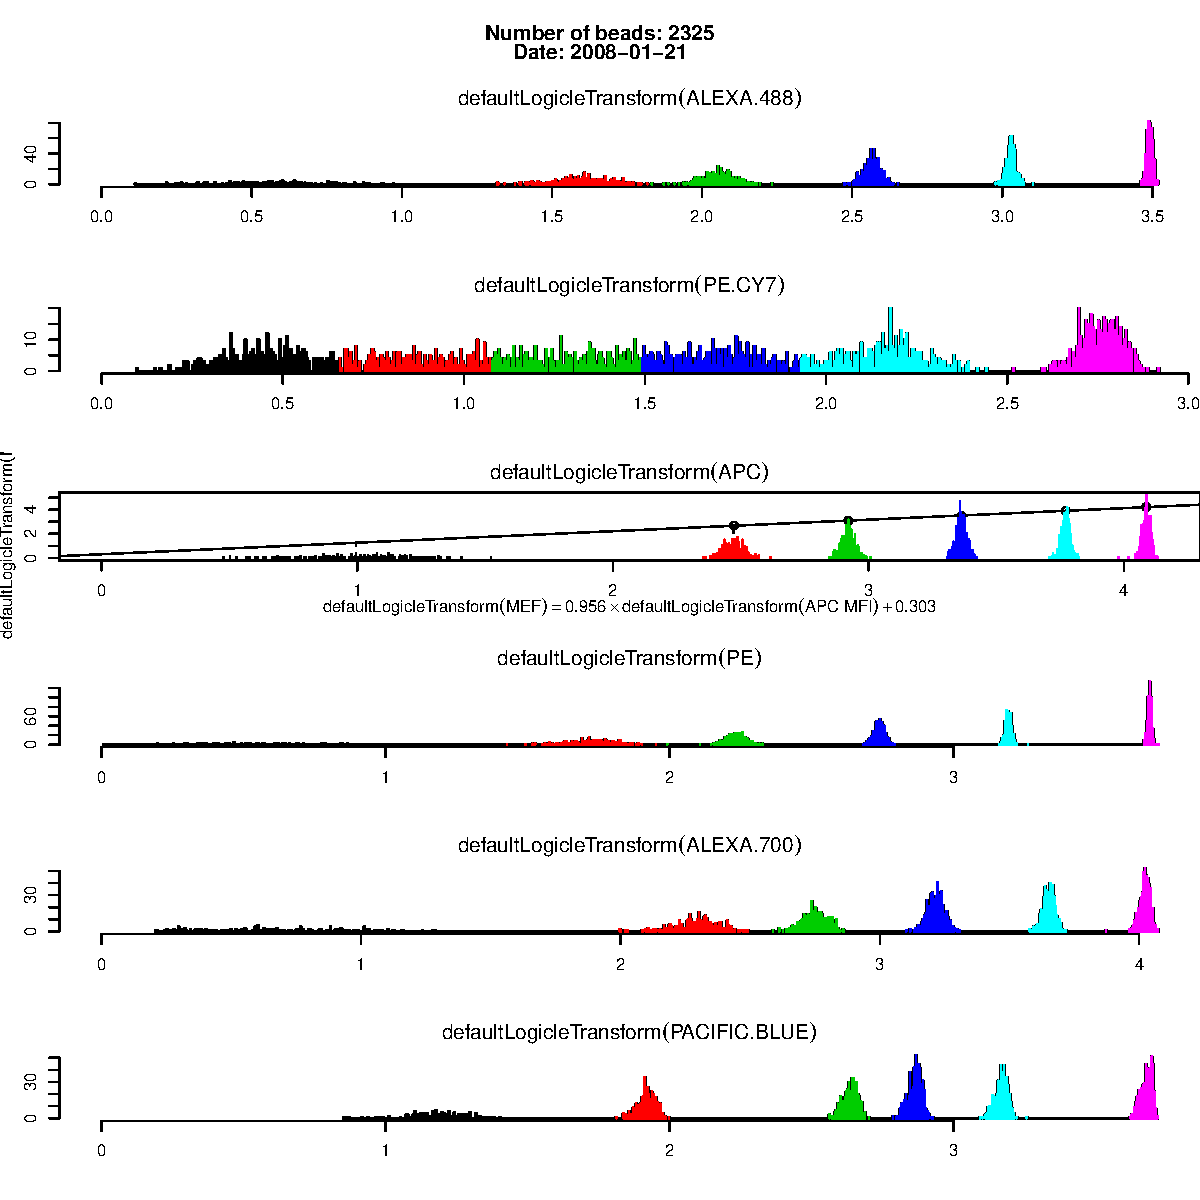
\includegraphics{./gbeads1plot}
  \caption{
  \label{gbeads1plot}
  Plot of \Robject{gbeads1}.
  APC gated beads day 1. We see tight clusters.
  The channel for \texttt{PE.CY7} is not tuned to pick up the signal hence in the noise.
  }
\end{figure}

%
\begin{figure}
  \centering
  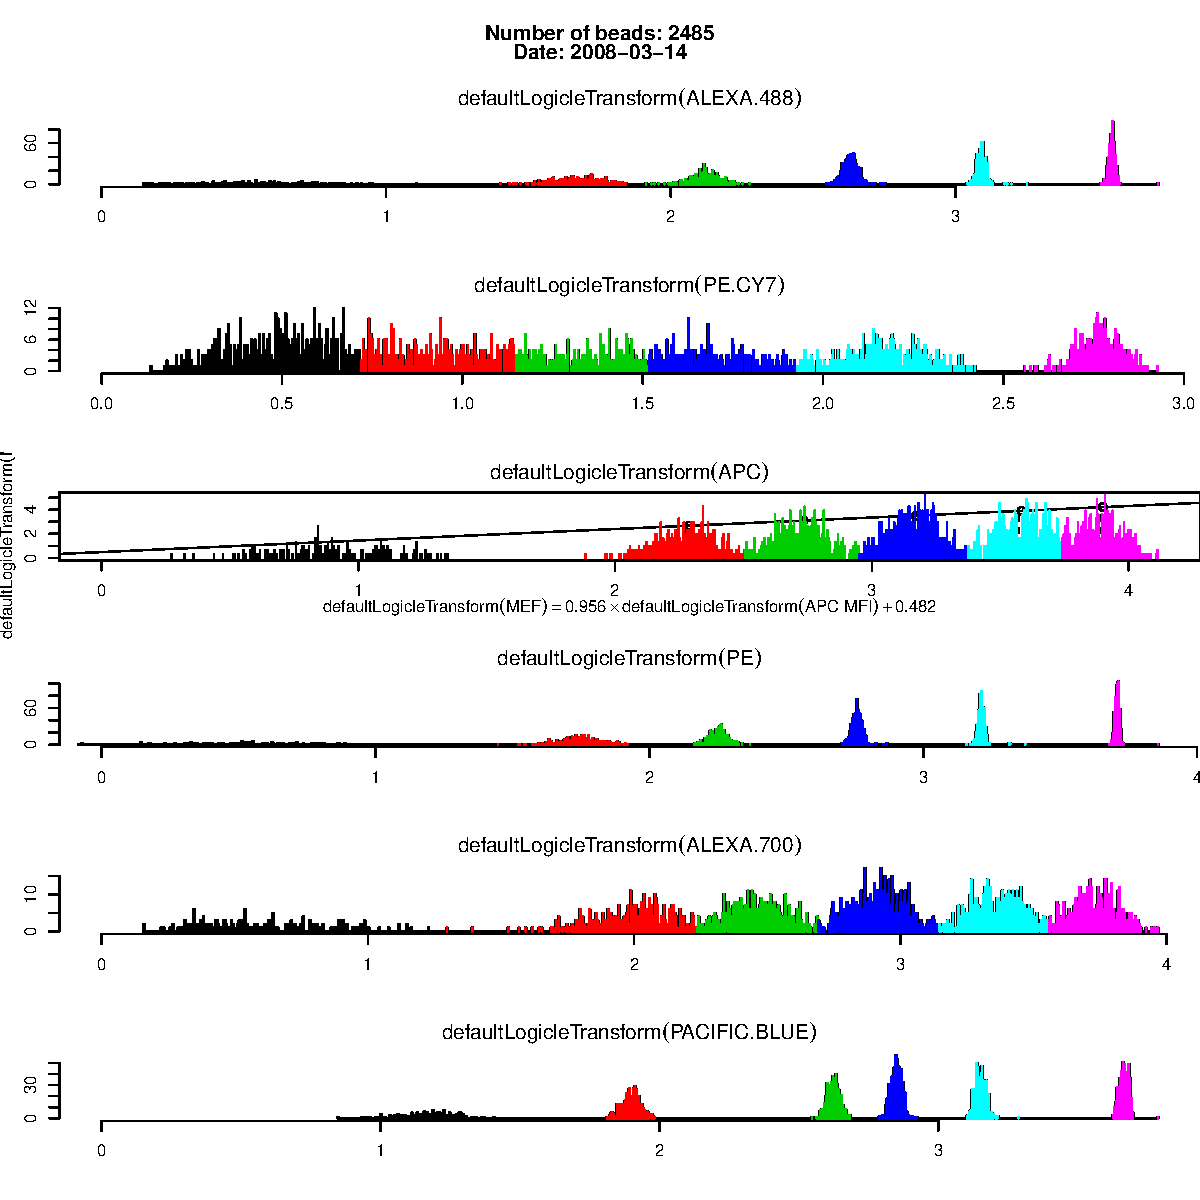
\includegraphics{./gbeads2plot}
  \caption{
  \label{gbeads2plot}
  Plot of \Robject{gbeads2}.
  APC gated beads day 2 the $\alpha$ is higher than on day 1 which implies higher background.
  The clusters are also far more noisy on this day than on the previous day.
  The channel for \texttt{PE.CY7} is not tuned to pick up the signal hence in the noise.
  }
\end{figure}

%
\begin{figure}
  \centering
  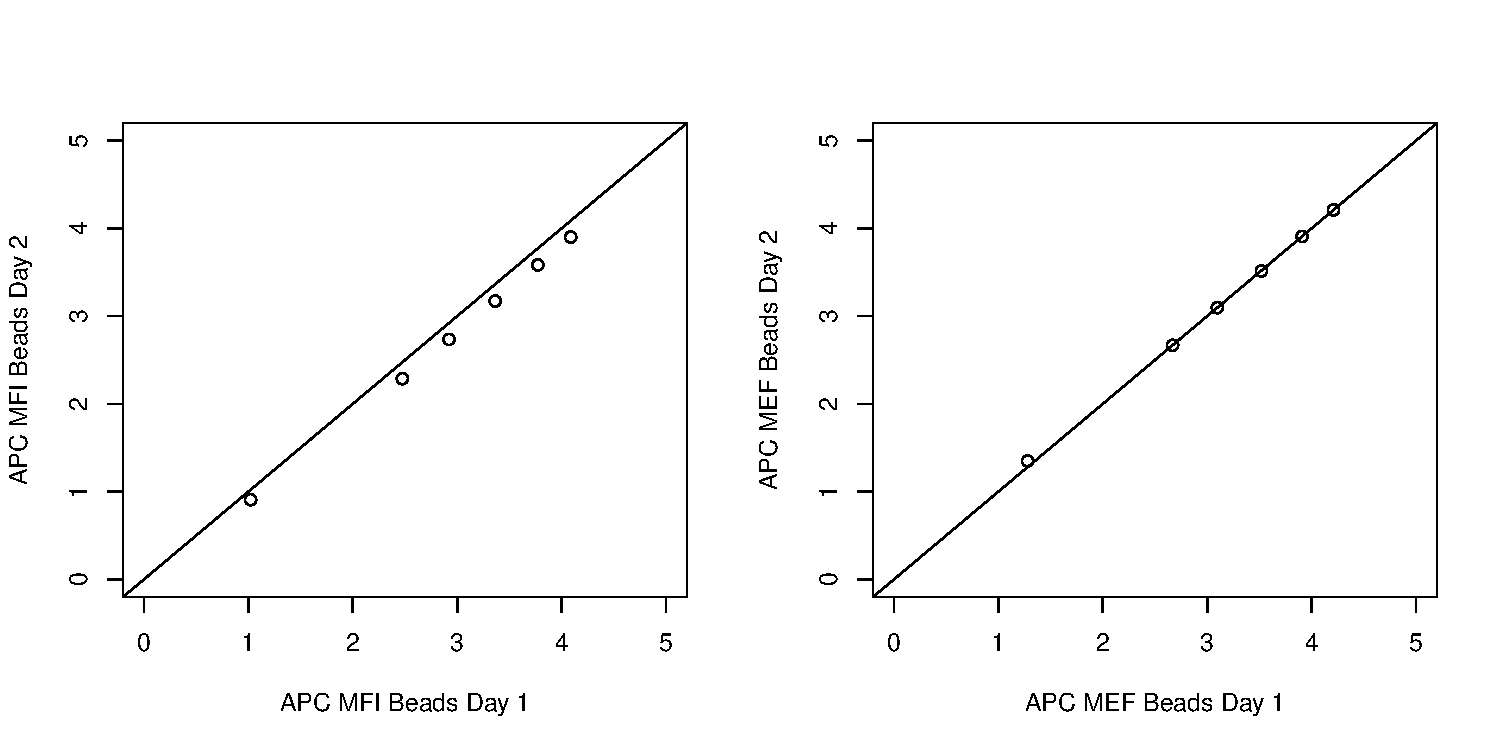
\includegraphics{./plotMEFrepeatability}
  \caption{
  \label{fig:absoluteNormalisation}
  The result of the MEF transform is to align the MFI of the five (non-blank) bead populations across days.
  Notice that that the alignment of the blank bead population is not perfect since it is not used in estimating the normalisation parameters.
  }
\end{figure}

%
\begin{figure}
  \centering
  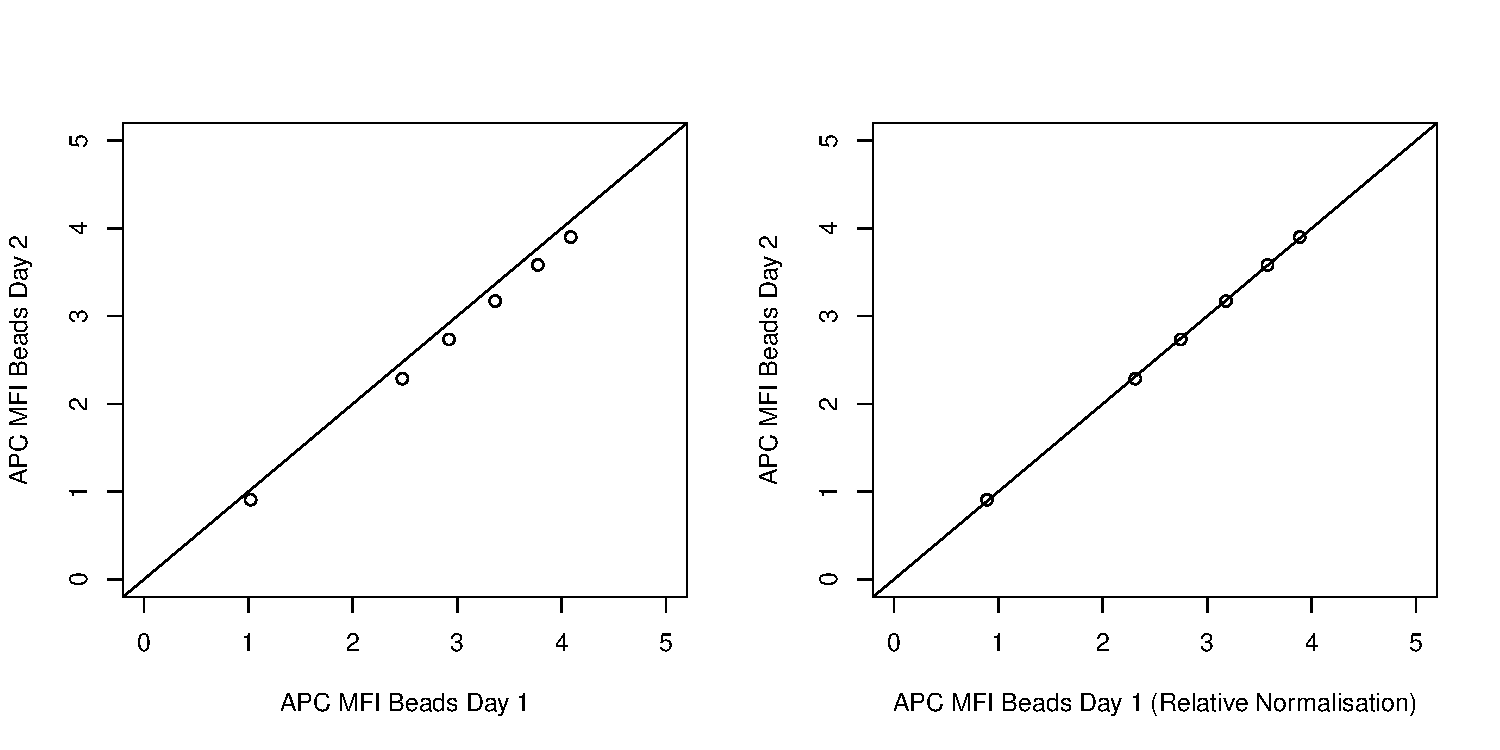
\includegraphics{./plotMFIrepeatability}
  \caption{
  \label{fig:relativeNormalisation}
  The result of the relative MFI transform is to align the MFI of the six bead populations across both days.
  Note that after relative normalisation, the MFIs from all bead populations are perfectly aligned.
  }
\end{figure}



\clearpage

\bibliographystyle{plainnat} 
\bibliography{beads}

\end{document}
